\documentclass[openany]{book}

\usepackage{fancyhdr}
\pagestyle{fancy}
% with this we ensure that the chapter and section
% headings are in lowercase.
\renewcommand{\chaptermark}[1]{%
\markboth{#1}{}}
\renewcommand{\sectionmark}[1]{%
\markright{\thesection\ #1}}
\fancyhf{}
% delete current header and footer
\fancyhead[LE,RO]{\bfseries\thepage}
\fancyhead[LO]{\bfseries\rightmark}
\fancyhead[RE]{\bfseries\leftmark}
\renewcommand{\headrulewidth}{0.5pt}
\renewcommand{\footrulewidth}{0pt}
\addtolength{\headheight}{0.5pt} % space for the rule
\fancypagestyle{plain}{%
\fancyhead{} % get rid of headers on plain pages
\renewcommand{\headrulewidth}{0pt} % and the line
}

\usepackage{tikz}
\usepackage[top=1in,bottom=1in,right=1in,left=1in]{geometry}

\usepackage{romannum}
\usepackage{fontspec}
% \setmainfont{Montserrat}
% \setmainfont{FiraMono-Regular}
% \setmainfont{FiraSans-Regular}
\setmainfont{SourceCodePro-Regular}
% \setmainfont{SourceSansPro-Regular}

\usepackage{xcolor}
\definecolor{mycyan}{RGB}{0,128,128}

\usepackage{amsmath} % American Math Society
\usepackage{amsthm} % Additional theorem functionality
\usepackage{amssymb} % Not necessarily part of asmmath but contains important characters such as Real number sign
\usepackage{IEEEtrantools}
\usepackage{latexsym} % \leadsto

% \renewcommand\qedsymbol{$\blacksquare$}
\DeclareMathOperator{\operator}{operator name}
\newcommand{\ud}{\, \mathrm{d}}

% Comment the following to have chapters numbered without interruption (numbering through parts)
% \makeatletter\@addtoreset{chapter}{part}\makeatother%

\title{My First \LaTeX{} Attempt}
\author{Trey Wilkinson}

% \theoremstyle{definition} % fat title, roman body
% \theoremstyle{plain} % fat title, italic body
% \theoremstyle{remark} % italic title, roman body

% \newtheorem{theorem}{Theorem}[chapter]
% \newtheorem{corollary}{Corollary}[theorem]
% \newtheorem{lemma}{Lemma}[theorem]
% \newtheorem*{remark}{Remark}

\usepackage{makeidx}
\makeindex
\usepackage[unicode=true]{hyperref}
\begin{document}
\maketitle
\tableofcontents

\part{Test}

%%%%%%%%%%%%%%%%%%%%%%%%%%%%%%%%%%%%%%%%%%%%%%%%%%%%%%%%%%%%%%%%%%%%%%%%%%%%%%%%
\chapter{Second chapter}
\textcolor{mycyan}{\href{https://youtube.com}{YouTube}}

\section{Typesetting}

\begin{table}[b]
    \centering\small
    \begin{tabular}{c r @{.} l}
        Pi expression & \multicolumn{2}{c}{Value} \\
        \hline
        $\pi$ & 3&1416 \\
        $\pi^\pi$ & 36&46 \\
        $(\pi^\pi)^\pi$ & 80662&7
    \end{tabular}
    \caption[Short caption]{Caption for $\pi$}
    \label{table:one}
\end{table}

\begin{proof}
    \begin{IEEEeqnarray}{+rCl+x*}
        \hat{x} & = & y \\
        \widehat{x} & = & z \\
        \therefore \quad y & = & z. \\
        &&& \qedhere \nonumber
    \end{IEEEeqnarray}
\end{proof}

% \begin{tabular}[pos]{l|r|p{50px} @{***}}
%     left align &  right align & text that is treated as a paragraph and wraps. \\ \cline{2-2}
%     one & two & three
% \end{tabular}

\subsection{Some math stuff}
\begin{equation}
    \tag{Math person}
    \tau\epsilon\chi \label{math:greek}
\end{equation}
% \\[10pt]
\[e=m \cdot c^2\]
\ref{math:greek}
Using \textbackslash smash\{equation\} ignores that equations height for line-height.

\begin{equation}
    \frac{d}{dx} f(x) = f'(x) = \lim_{h \to 0} \frac{f(x + h) - f(x)}{h}
\end{equation}
\begin{equation}
    x^2 \geq 0\qquad \forall \text{(for all) } x \in \mathbb{R}
\end{equation}
The command \verb|\text{text}| can be used to add normal text within equations.

\begin{align}
    \binom{n}{k} \qquad \bar{xyz} \quad & \quad \vec{xyz} \qquad \overrightarrow{xyz} \\
    0.\overline{3} & \stackrel{\leftrightarrow}{\stackrel{\equiv}{\Leftrightarrow}} \underline{\underline{\underline{1/3}}} \\
    & \underbrace{\cdots\ldots\vdots\overbrace{\ddots\cdot}^{dots}}_{\text{underneat}}
\end{align}
\begin{multline*}
    \left.(\left(\left[\int^n_{\substack{0<i<n\\i \subseteq n}}\right]\right)\right) \\
    \int \iint \iiint \iiiint
    \int_{\mathbb{C}^n} \\
    \{\big\{\Big\{\bigg\{\Bigg\{ \\
    \|\big\|\Big\|\bigg\|\Bigg\| \\
    \Downarrow\big\Downarrow\Big\Downarrow\bigg\Downarrow\Bigg\Downarrow \\
\end{multline*}
\pageref{table:one}
\begin{IEEEeqnarray}{rCll}
    a & = & b + c + d & \qquad \text{ Some notes} \\
    & = & a + b + c & \qquad \text{ Some more notes}\\
    && \negmedspace{} + d + e
\end{IEEEeqnarray}

\begin{equation*}
    \mathbf{x} = \left[ \begin{array}{ccc}
        x_0 & x_1 & \ldots \\
        x_2 & x_3 & \ldots \\
        \vdots & \vdots & \ddots
    \end{array}
    \right]
    \begin{matrix}
        1 & 2 \\ 3 & \phantom{1234}4
    \end{matrix}
    \begin{bmatrix} % matrix, bmatrix, Bmatrix, pmatrix, vmatrix, Vmatrix
        1 & 2 & 3 \\ 4 & 5 & 6 \\ 7 & 8 & 9
    \end{bmatrix}
\end{equation*}
% {\let\cleardoublepage\clearpage\listoftables}

\section{Specialties}

Hi~\cite{ae} has said

Hi\cite{tw} has said

Hi \cite{tw} has said

\begin{thebibliography}{99}
    \bibitem{ae} Albert Einstein
    \bibitem{tw} Trey Wilkinson
\end{thebibliography}

\section{Producing Mathematical Graphics}
\setlength{\unitlength}{1mm}
\begin{picture}(60,40)
    \put(20,30){\circle{2}}
    \put(20,30){\circle{4}}
    \put(20,30){\circle{6}}
    \put(20,30){\circle{8}}
    \put(20,30){\circle{10}}
    \put(20,20){$\sqrt[^3]{x^2+y^2}$}
\end{picture}

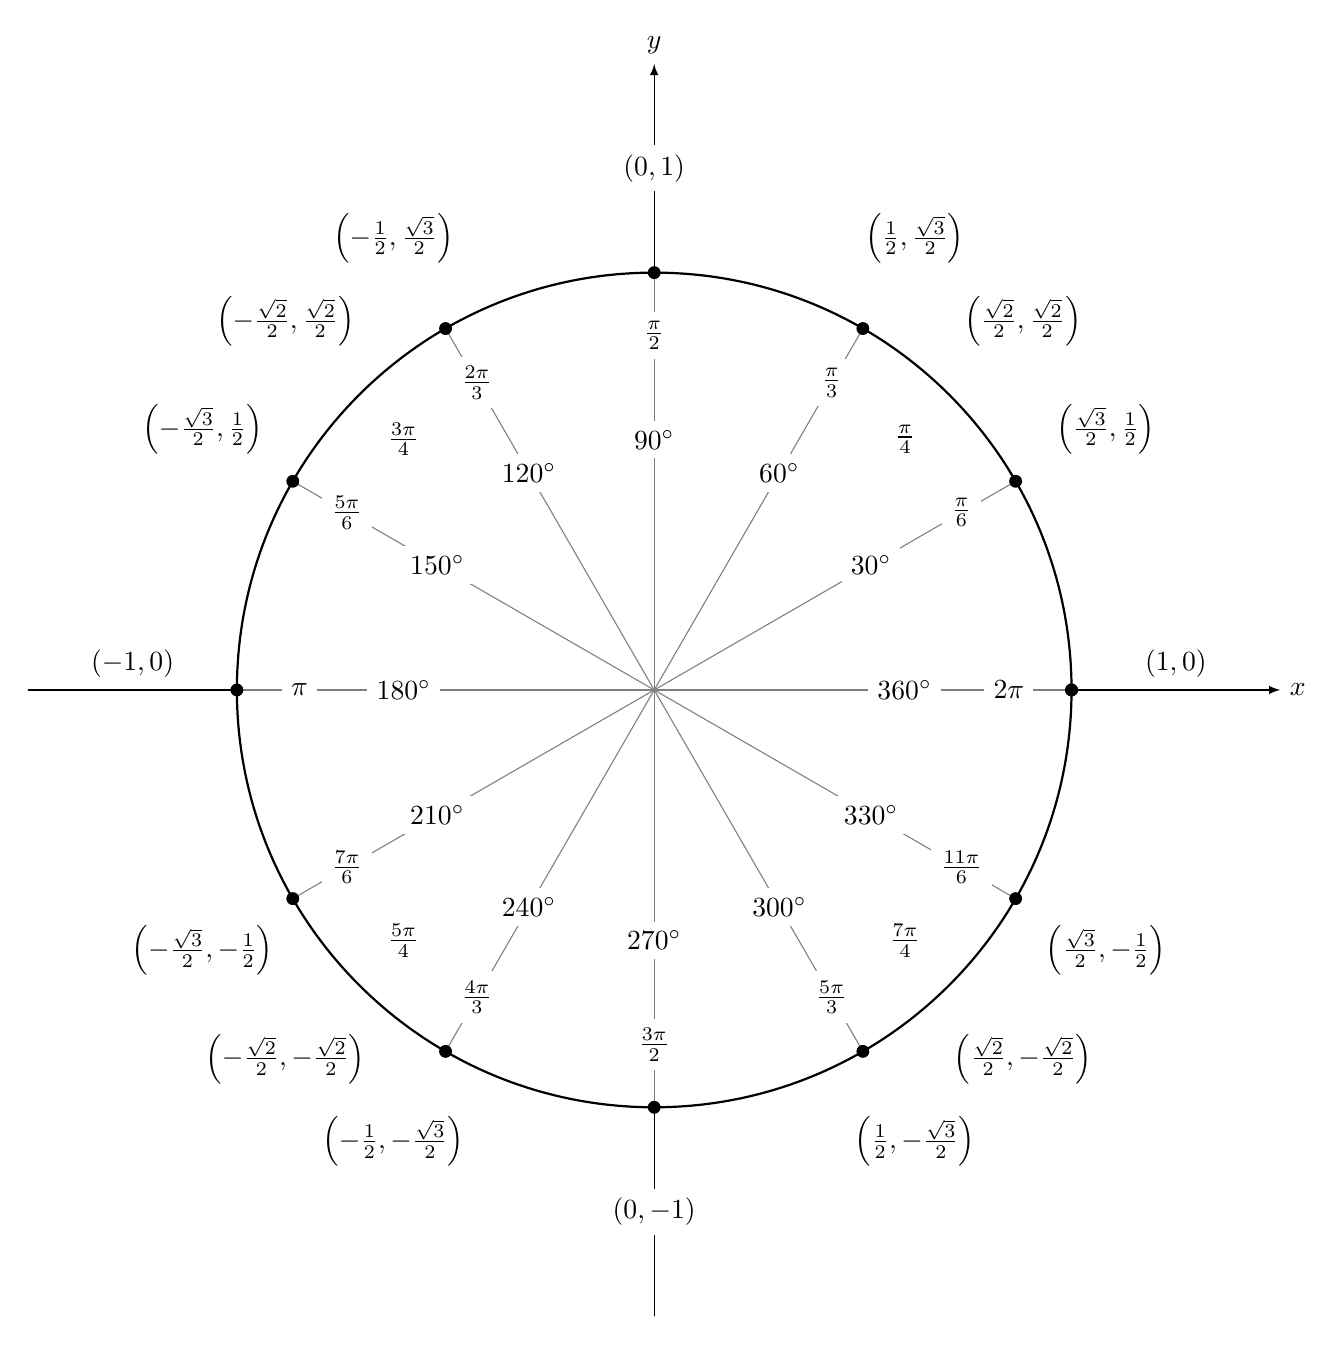
\begin{tikzpicture}[scale=5.3,cap=round,>=latex]
    % draw the coordinates
    \draw[->] (-1.5cm,0cm) -- (1.5cm,0cm) node[right,fill=white] {$x$};
    \draw[->] (0cm,-1.5cm) -- (0cm,1.5cm) node[above,fill=white] {$y$};

    % draw the unit circle
    \draw[thick] (0cm,0cm) circle(1cm);

    \foreach \x in {0,30,...,360} {
            % lines from center to point
            \draw[gray] (0cm,0cm) -- (\x:1cm);
            % dots at each point
            \filldraw[black] (\x:1cm) circle(0.4pt);
            % draw each angle in degrees
            \draw (\x:0.6cm) node[fill=white] {$\x^\circ$};
    }

    % draw each angle in radians
    \foreach \x/\xtext in {
        30/\frac{\pi}{6},
        45/\frac{\pi}{4},
        60/\frac{\pi}{3},
        90/\frac{\pi}{2},
        120/\frac{2\pi}{3},
        135/\frac{3\pi}{4},
        150/\frac{5\pi}{6},
        180/\pi,
        210/\frac{7\pi}{6},
        225/\frac{5\pi}{4},
        240/\frac{4\pi}{3},
        270/\frac{3\pi}{2},
        300/\frac{5\pi}{3},
        315/\frac{7\pi}{4},
        330/\frac{11\pi}{6},
        360/2\pi}
            \draw (\x:0.85cm) node[fill=white] {$\xtext$};

    \foreach \x/\xtext/\y in {
        % the coordinates for the first quadrant
        30/\frac{\sqrt{3}}{2}/\frac{1}{2},
        45/\frac{\sqrt{2}}{2}/\frac{\sqrt{2}}{2},
        60/\frac{1}{2}/\frac{\sqrt{3}}{2},
        % the coordinates for the second quadrant
        150/-\frac{\sqrt{3}}{2}/\frac{1}{2},
        135/-\frac{\sqrt{2}}{2}/\frac{\sqrt{2}}{2},
        120/-\frac{1}{2}/\frac{\sqrt{3}}{2},
        % the coordinates for the third quadrant
        210/-\frac{\sqrt{3}}{2}/-\frac{1}{2},
        225/-\frac{\sqrt{2}}{2}/-\frac{\sqrt{2}}{2},
        240/-\frac{1}{2}/-\frac{\sqrt{3}}{2},
        % the coordinates for the fourth quadrant
        330/\frac{\sqrt{3}}{2}/-\frac{1}{2},
        315/\frac{\sqrt{2}}{2}/-\frac{\sqrt{2}}{2},
        300/\frac{1}{2}/-\frac{\sqrt{3}}{2}}
            \draw (\x:1.25cm) node[fill=white] {$\left(\xtext,\y\right)$};

    % draw the horizontal and vertical coordinates
    % the placement is better this way
    \draw (-1.25cm,0cm) node[above=1pt] {$(-1,0)$}
          (1.25cm,0cm)  node[above=1pt] {$(1,0)$}
          (0cm,-1.25cm) node[fill=white] {$(0,-1)$}
          (0cm,1.25cm)  node[fill=white] {$(0,1)$};
\end{tikzpicture}

\section{Customising \LaTeX}


\chapter{Last chapter}

\part{Math}
\chapter{Logic}
\section{Proof Techniques}
\subsection{Strategies}
\begin{enumerate}
    \item \textbf{Make a start.} Anything is better than nothing. Start piecing together facts.
    \item \textbf{Identity assumption(s) and conclusion.} Helps you identitfy what definitions/theorems/etc. could be used in the proof.
    \item \textbf{Try working backwards and/or fill the middle of the proof.} The goal is to find steps which lead from the assumptions, from which the conclusion follows.
    \item \textbf{Understand the concepts.} Understand the definitions and theorems by heart.
    \item \textbf{Determine the logical form of the statement.} The logical form may help you know how to proceed.
\end{enumerate}

\chapter{Algebra}
\section{Algebra: 0}
$I \rightarrow II \rightarrow III \rightarrow V \rightarrow VI \rightarrow VIII \rightarrow IX$
\\ (Pass through $IV$ and $VII$ on first pass)

\subsection{I. Preliminaries: Set theory and categories}
\subsection{II. Groups, first encounter}
\subsection{III. Rings and modules}
\subsection{VII. Fields}
\subsection{IX. Homological Algebra}

\chapter{Analysis}
\section{Real Analysis}
\section{Complex Analysis}
\section{Functional Analysis}
\section{Tensor Analysis}

\end{document}

%%%%%%%%%%%%%%%%%%%%%%%%%%%%%%%%%%%%%%%%%%%%%%%%%%%%%%%%%%%%%%%%%%%%%%%%%%%%%%%%

\documentclass[10pt, letterpaper]{book}
\usepackage[unicode=true]{hyperref}
\usepackage{graphicx}
\usepackage{amsmath}
\usepackage{syntonly}
% \syntaxonly % only checks for syntax

\graphicspath{ {images/} }

\title{This is my first text document.}
\date{November 24, 2020}
\author{Trey Wilkinson}
\setcounter{tocdepth}{4} % sets the depth of table of contents
\newcommand{\testme}[2]{
    \begin{enumerate}
        \item #1
        \item #2
    \end{enumerate}
}


\begin{document}
\maketitle

\chapter*{Abstract}
    This is a outline to some topics.
    First document using \LaTeX{}\ldots{}
\tableofcontents
\part{Test}
\chapter{Chapter One}
\section{Section One}
    \label{section:one}

%     \begin{figure}[h]
%         \label{one:synth}
%         \centering
%         \includegraphics[width=0.50\textwidth]{synthwave}
%         \caption{some Figure}
%     \end{figure}
%     This is some ref to the image \ref{one:synth}, the page is on \pageref{one:synth}

An \textbf{equation} \emph{as} \underline{follows}: $\forall A. \exists e. (e = A)$ can be used to describe things. L\-ong\-word\-thatisrighthere.
\mbox{mobx(will not be hypheanated)} \fbox{fbox}.\footnote{This is my footnote}

``As simple as possible and no simpler.'' \emph{Einstein}
\\ x-x x--x x---x $-x$ $\sim x^\circ$ \\ff vs f\mbox{f}\\X.~vs. X\\G\"odels or \`\i or \'\i

\begin{quotation}
    This is a long quotation.

    That spans multiple lines.
\end{quotation}

Verbatim
\begin{verbatim*}
The star shows spaces
2834u019835 sadklfj 58132u4089235 asdkfjaslkdf\easdfkj 3258u9$ $
\end{verbatim*}

\verb|a893%51234\eavser r$$ $$ $alsfsdlfkjasdlfk|
$$
e = m \cdot c^2 \; ,
\sum \sum_{k=1}^{n}
$$
\[ T^{i_1 i_2 \dots i_p}_{j_1 j_2 \dots j_q} = T(x^{i_1},\dots,x^{i_p},e_{j_1},\dots,e_{j_q}) \]

\[ \int_0^1 \frac{dx}{e^x} =  \frac{e-1}{e} \]

Mathematical operators are prefixed with a backslash as $\sin(\beta)$, $\cos(\Omega)$, $\log(x)$ etc.

\section{two}
\# \$ - \{ \} \% \^ \_{} are special characters.
The \% is used for comments.
\TeX{} with a space and \TeX with no space

\section*{Section not toc}
\begin{center}
    \begin{enumerate}
        \item part (does not modify numbering)
        \item [item1] chapter
        \item [item5] section
        \item subsection
        \item subsubsection
        \item paragraph
        \item subparagraph
    \end{enumerate}
\end{center}
\pageref{section:one}

\section{Books}
\begin{description}
    \item[frontmatter]{Roman numeral page numbering.}
    \item[mainmatter]{Arabig page numbering.}
    \item[appendix]{Start of additional material in book. Chapters numbered with lettered.}
    \item [backmatter]{For bibliography and stuff. }
\end{description}

\ref{table:groups}

\addcontentsline{toc}{section}{GROUPS}
\subsection{Group Structures}
\begin{table}[h!]
    \centering
    \begin{tabular}{|l|c|c|c|c|c|}
        \hline
        Group-like structures & Totality & Associativity & Identity & Invertibility & Commutativity \\
        \hline
        Semigroupoid          &     -    &        +      &     -    &        -      &        -  \\
        Small-Category        &     -    &        +      &     +    &        -      &        -  \\
        Groupoid              &     -    &        +      &     +    &        +      &        -  \\
        Magma                 &     +    &        -      &     -    &        -      &        -  \\
        Quasigroup            &     +    &        -      &     -    &        +      &        -  \\
        Unital-Magma          &     +    &        -      &     +    &        -      &        -  \\
        Loop                  &     +    &        -      &     +    &        +      &        -  \\
        Semigroup             &     +    &        +      &     -    &        -      &        -  \\
        Inverse-Semigroup     &     +    &        +      &     -    &        +      &        -  \\
        Monoid                &     +    &        +      &     +    &        -      &        -  \\
        Commutative-monoid    &     +    &        +      &     +    &        -      &        +  \\
        Group                 &     +    &        +      &     +    &        +      &        -  \\
        Abelian-group         &     +    &        +      &     +    &        +      &        +  \\
        \hline
    \end{tabular}
    \label{table:groups}
    \caption{Group-like structures}

\end{table}

\end{document}
